\subsection{Strong Interactions}
\label{sec:Intro_QCD}

\begin{figure}[htb]
  \begin{center}
    {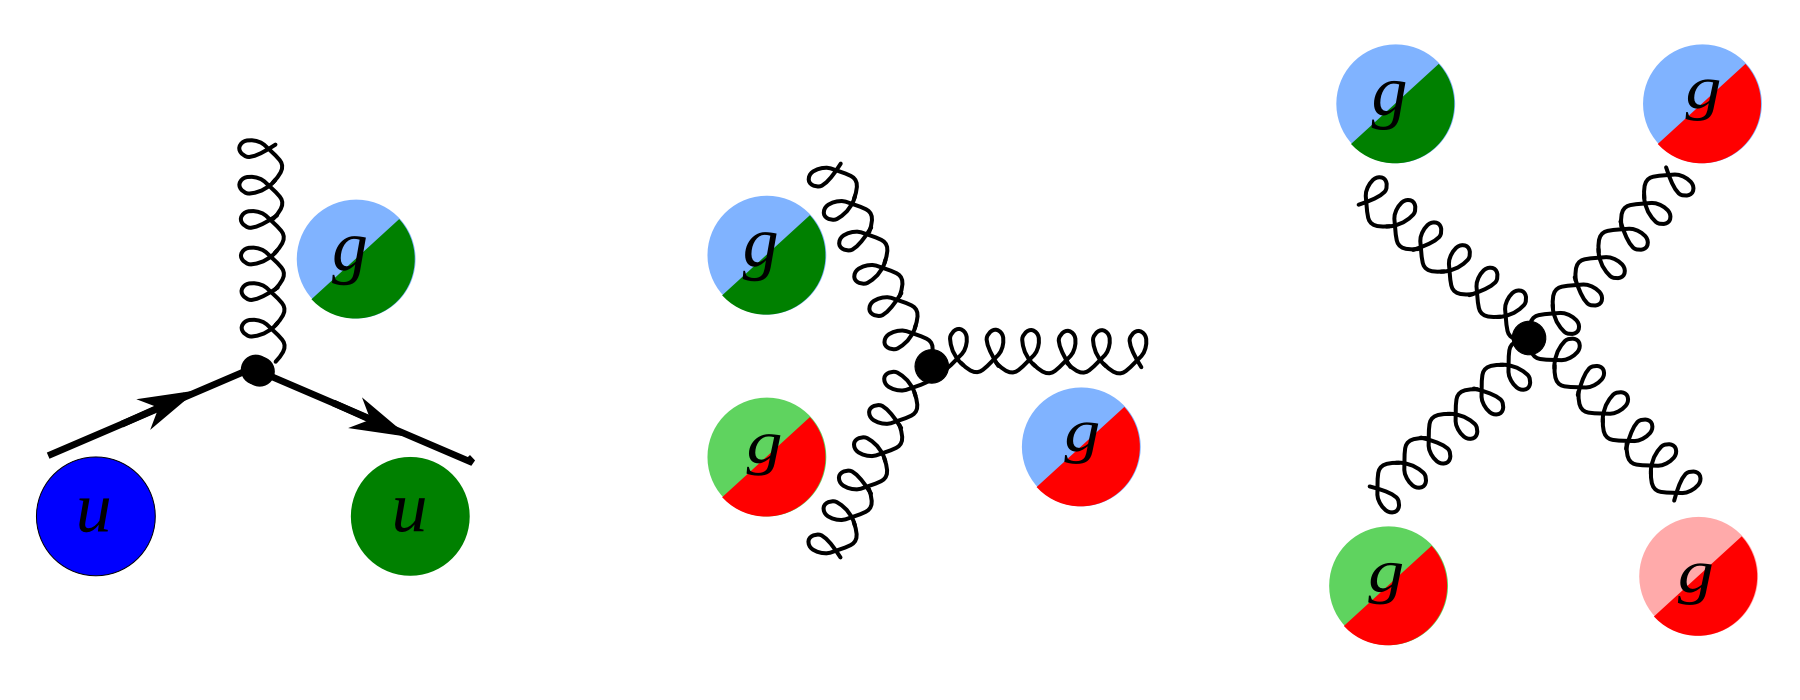
\includegraphics[width=0.80\textwidth]{../figs/Intro/feynmStrong.png}}
    \caption{Elementary processes of strong interations}
    \label{fig:feynmStrong}
  \end{center}
\end{figure}


The third fundamental force after the electromagnetic and weak ones is the strong force. The strong force is responsible for gluing protons and neutrons together in the nuclei as well as for forming protons and neutrons themselves. The strong interactions occur by exchanging gluons which are spin-one massless electrically neutral particles.  \\

The elementary strong processes are shown in Fig. \ref{fig:feynmStrong}. There are three elementary processes: $qqg$, $ggg$ and $gggg$, all are involving particles with color charges. Thus, gluons couple to quarks and self-couple. Color charges must be conserved at each elementary process of the strong interaction. Each quark possesses one of three colors at a time, and there are eight types of gluons to cover all possible color exchanges. \\

The coupling constant of the strong interaction depends on a distance between interacting particles: it becomes larger as the distance becomes larger and smaller as the distance becomes smaller. As the distance approaches zero, the coupling constant approaches zero too, and, thus, in the asymptotic limit two quarks located at the same place do not interact. This property is called asymptotic freedom.\\

On the other hand, when the distance between quarks becomes larger, the coupling constant also becomes larger. This property confines quarks to always stay in the color neutral combinations (hadrons), it forbids the existence of free quarks. A combination becomes color neutral when there is the same amount of color and anticolor or if there is the same amount of each of the three colors.  Thus, mesons are comprised of a quark and an antiquark with the opposite color charges, and baryons are comprised of three quarks: red, green and blue one. Examples of baryons include such well-known particles as a proton and a neutron.\\

The asymptotic freedom and the confinement are properties that are specific for strong interactions. The theory of strong interactions is called the quantum chromodymanics (QCD) which is a quantum field theory invariant under $SU(3)$ color transformations. When the coupling constant is much less than one $\alpha_s \ll 1$, the perturbative approach can be used to compute observables.\\

The W$\gamma$ process being measured in this dissertation is not intended to test QCD, but a good understanding of QCD is essential for performing this measurement because the QCD corrections to the Feynman diagrams of the process are large and have to be taken into account when producing simulation. In addition, QCD describes the dynamics of quarks and gluons within colliding protons and predicts probabilities of one or another quark-antiquark pair to interact. Physics of proton-proton collisions is discussed in the Ch.~\ref{sec:Intro_ppCollisions}. \\

% Possible QCD corrections include quark-gluon loops at any of three quark lines as well as exchanges of gluons between different quark lines. 
